\subsubsection{Wi-Fi}%
\label{sec:wifi-test}
%
After the implementation of the Wi-Fi module forementioned in \ref{sec:wifi-implem-connection}, one needed to perform tests in the connection between two smartphones and also between the smartphone and the \gls{rvvs}. These tests will be discussed in the following sections. 
%
\subsubsection{Wi-Fi: Smartphone-Smartphone}
\label{sec:wifi-phone-phone}
%
For the tests related to the smartphone's wifi module, one tested the connection setup (figure \ref{fig:phone-wifi-setup}) and the capability of message exchange (figure \ref{fig:phone-wifi-messages}). Firstly, Wi-Fi must be enabled using the enable Wi-Fi button, accepting the request to turn it on. Next, one should press the Wifi Discover button, advancing to the subsequent screen, where a list of the available devices for connection is displayed. The green text on top of the screen refers to the current status of the application in terms of the wifi setup. When the user presses a list from the list, a request pop-up for Wi-Fi connection is presented. Accepting the request, the status changes to connected and the host and client are identified. Lastly, one tested sending and receiving messages from a smartphone to another smartphone by simply trying to press a WIFI MSG button to send a specific message, but due to deadline proximity, this feature wasn't functional and the Wi-Fi smartphone-\gls{rvvs} tests were abandoned. 
%
\begin{figure}[!ht]
\centering
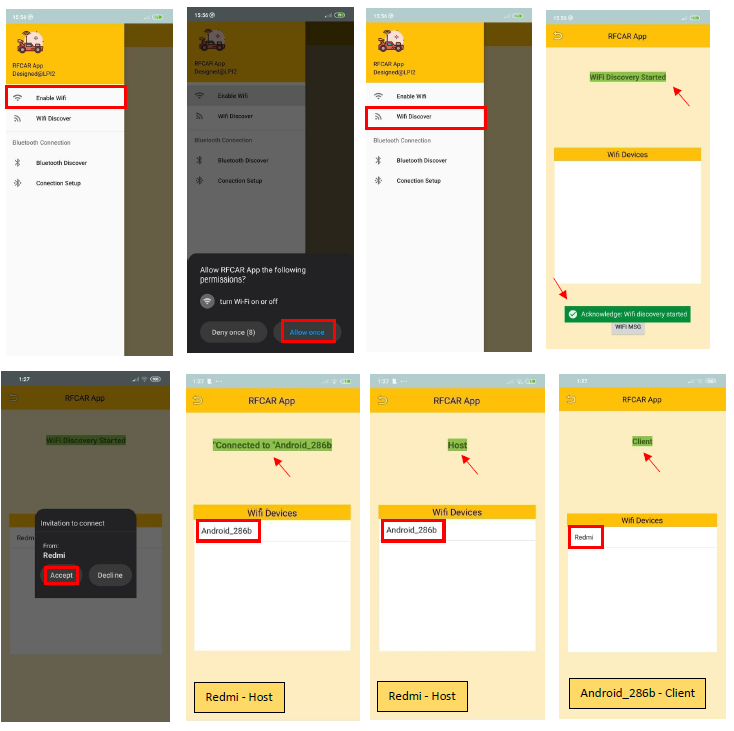
\includegraphics[width=\textwidth]{img/phone-wifi-setup.png}
\caption{\label{fig:phone-wifi-setup}Wi-Fi connection setup tests}
\end{figure}
%
\begin{figure}[!ht]
\centering
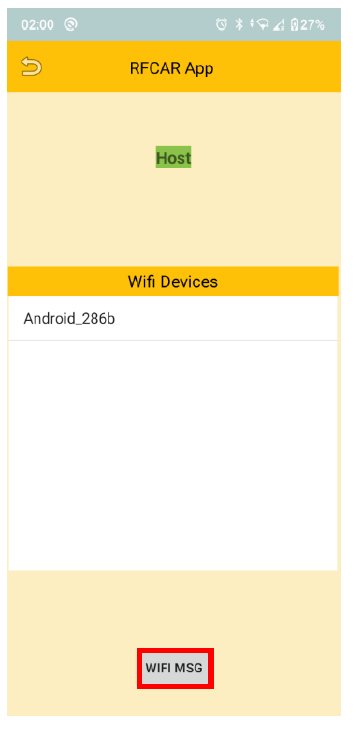
\includegraphics[width=0.3\textwidth]{img/phone-wifi-message.png}
\caption{\label{fig:phone-wifi-messages}Wi-Fi message exchange tests}
\end{figure}
%
%\subsubsection{Wi-Fi: Smartphone-RVVS}
%\label{sec:wifi-phone-rvvs}
%